\section{Introduction}

For linear time-invariant systems, the nonparametric impulse response model gives a complete and intuitive description of the system space. As a consequence, its truncated FIR form is the model structure of choice in many modern regularized estimation procedures, which were discussed in Chapter \ref{chap:2}. When broadening our scope to \emph{nonlinear} time-invariant systems, an analogous nonparametric representation is known as the Volterra series \cite{Schetzen1980}, named for mathematician Vito Volterra and his pioneering work on analytic functionals \cite{Volterra1930}. 

In much the same way that linear functions are just one term in the Taylor series description of nonlinear static functions, the linear impulse response becomes one term in a series of multi-dimensional impulse responses, which together form the Volterra series description of nonlinear dynamical systems. Each successive term in the series contains one additional dimension in its impulse response, and represents a single `nonlinear order' of the system. For example, the next term after the linear impulse is a 2-dimensional impulse response which describes all 2\textsuperscript{nd} order (quadratic) nonlinear behaviour in the system. In theory, the Volterra series has both infinite terms and infinite memory lengths within each term. The series is typically defined in the time domain, since this is the domain of an impulse response, however there are also equivalent frequency domain representations \cite{Schetzen1980}, \cite{Lang2005}, \cite{Lang2007} which can be obtained using appropriate Fourier transformations. Furthermore, all representations of the Volterra series can be described using continuous- or discrete-time models.

In practice, for data-driven modeling and control, the Volterra series must be truncated such that there is a finite maximum nonlinear order, and each impulse response term has finite memory length. It has been shown in \cite{Boyd1985} that a truncated, finite memory Volterra series model can approximate any fading memory nonlinear system arbitrarily well. The fading memory condition is somewhat similar to a stability condition in linear systems, requiring that the current system output not be influenced by input signals applied in the remote past. This will also exclude nonlinear system classes which exhibit, for example, hysteresis or non-unique steady-states. The fading memory condition still leaves an incredibly broad set of systems which can be universally approximated, along with many systems which can be approximated locally within a small region of some stable equilibrium point.

The extreme versatility of Volterra series models in representing nonlinear systems will motivate the use of such models in this thesis. In particular, the identification of nonlinear systems can be performed with very little prior knowledge, requiring user selections only for the maximum nonlinear order and memory lengths. Due to the multidimensional nature of the series, however, the model requires large numbers of parameters to be estimated, and this number grows rapidly with memory length and series order. From an identification perspective, large numbers of parameters means high covariance and MSE in the resulting estimates, particularly when the input/output data length is low or measurement noise is significant. There are also implications on the computational and memory requirements when considering a large parameter space. Such complications have historically restricted the use of classical estimators on Volterra series, and only in the most recent decades have new techniques emerged which enable more widespread use of the series in data-driven modeling. Some of these techniques will be discussed in Sections \ref{sec:VolterraID_History} and \ref{sec:RegVolterraTD}. 

\section{Discrete-time representations}
\label{sec:DTrepresentations_Volterra}

While the continuous-time Volterra series is a useful concept in systems theory, the nature of sampled data and nonparametric estimation dictates that we use discrete-time models for estimation and control. In the case where the system is excited by a piecewise constant input over the sampling periods, an explicit relationship between the discrete- and continuous-time models can be established \cite{Middleton1990}. Thus, we will restrict our focus in this thesis to the discrete-time definitions of Volterra series and its related expansions. Essentially, the only difference between these definitions and their continuous-time equivalents found in e.g. \cite{Schetzen1980} is the use of summations in place of continuous integrals. Naturally, the series terms also change from being continuously defined, to being defined only at integer values of their input arguments. The time and frequency domain representations are defined below.

\subsection{Time domain representation}

The Volterra series is most often expressed in the time domain, where its discrete-time representation can be given as,
\begin{align}
y^0(t) &= h_0 + \sum_{m=1}^M y_m(t), \label{eq:VolterraTimeDomainOutput} \\
y_m(t) &= \sum_{\tau_1 = 0}^{n_m-1} \hdots \sum_{\tau_m=0}^{n_m-1} h_m(\tau_1, \hdots, \tau_m) \prod_{\tau=\tau_1}^{\tau_m} u(t-\tau), \label{eq:VolterraConvolutionDefn}
\end{align}
where $u(t)$ and $y^0(t)$ denote the true system input and output respectively, $h_0 \in \mathbb{R}$ is a constant offset, and $y_m(t)$ is the output contribution from the $m$\textsuperscript{th} nonlinear order, up to some maximum series order, $M$. These output contributions are formed via the $m$-dimensional convolution in (\ref{eq:VolterraConvolutionDefn}), where $h_m(\tau_1, \hdots, \tau_m)$ is the $m$\textsuperscript{th} term of the Volterra series, $\tau_i$ is the $i$\textsuperscript{th} lag variable for the term, and $n_m$ is its memory length.

The series terms, $h_m$, are commonly referred to as \emph{Volterra kernels}, where the $m$\textsuperscript{th} kernel is an $m$-dimensional impulse response. It is these kernels which must be estimated for a Volterra series model. It should be noted that the 1\textsuperscript{st} order contribution, $y_1(t)$, is nothing more than the FIR model from (\ref{eq:FIRdefn}), and the corresponding Volterra kernel $h_1(\tau_1)$ behaves like a linear impulse response. 

A visual depiction of the time domain series is provided in Figure \ref{fig:VolterraSeriesVisualised} for the first four terms, showing the increase in dimension and complexity with each successive kernel.

\begin{figure}[h]
\centering
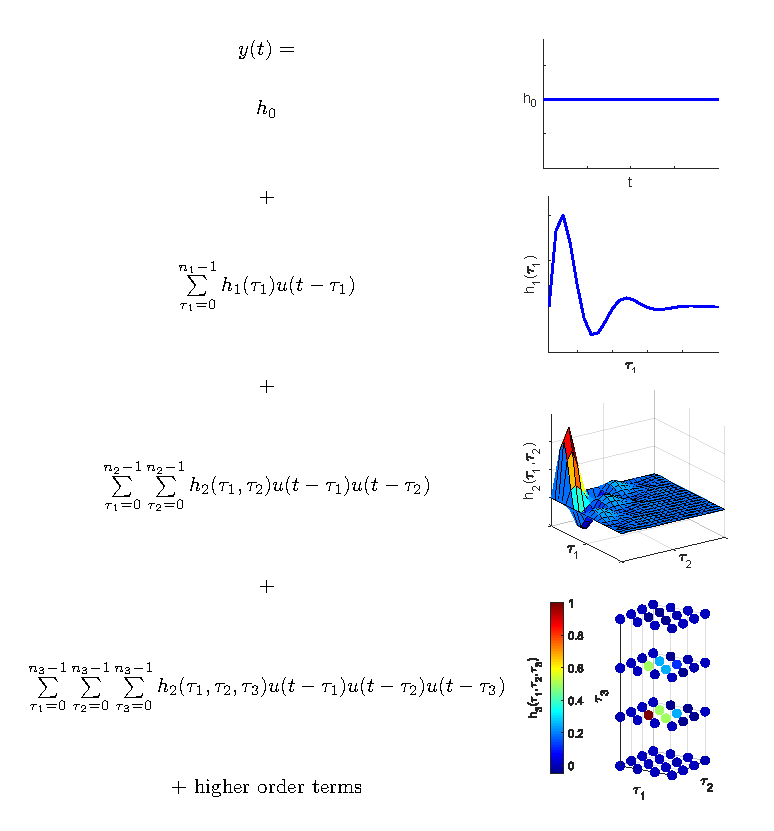
\includegraphics[width=0.9\textwidth]{Chapter3_VolterraSeries/PictorialSeries.pdf}
\caption{A visual example of the Volterra series for the first four terms}
\label{fig:VolterraSeriesVisualised}
\end{figure}

\subsection{Frequency domain representations}

The Volterra series can also be expressed in the frequency domain, with a number of competing representations available in the literature \cite{Cheng2017}. In their discrete-time form, all of these representations require an assumption that the system is in steady state. The assumption implies that an $N$-periodic (i.e. periodic with period $N$) input signal has been applied for a sufficiently long time so that the output is also $N$-periodic and free of transients. Then, for some $N$-sample measurement window, we can express the system input and output spectra, $U(k)$ and $Y^0(k)$ for $k=0,1,\hdots,N-1$, as the Discrete Fourier Transform (DFT) of their corresponding $N$-sample time domain signals $u(t)$ and $y^0(t)$. The relationship between these two steady state spectra will constitute the frequency domain model.

While each frequency domain structure has its own unique benefits, the most natural extension from the time domain series is a Generalized Frequency Response Function (GFRF) model. First derived in \cite{George1959}, the GFRF model is obtained via multidimensional Fourier transforms on each time domain series term. In discrete-time, the mathematical description is given by,
\begin{equation}
\begin{split}
Y^0(k) &= H_0(k) + \sum_{m=1}^{M} Y_m(k),  \\
Y_m(k) &= \frac{1}{N^{m-1}} \sum_{k_1 + \hdots + k_m = k} H_m(k_1, \hdots,k_m) \prod_{i=1}^{m} U(k_i), 
\end{split}
\label{eqn:GFRFoutputeqn}
\end{equation}
where $H_0(k) = h_0 \delta(k)$ is a zero frequency component from the constant offset $h_0$, $H_m(k_1, \hdots,k_m)$ is the $m$\textsuperscript{th} order GFRF term, and $k_i$ are discrete frequency variables. The GFRFs, $H_m$, are related to their equivalent $m$\textsuperscript{th} order time domain kernel, $h_m$, via multidimensional DFTs, i.e.
\begin{equation}
\label{eqn:GFRF_Transform}
H_m(k_1, \hdots,k_m) = \sum_{\tau_1=0}^{n_m - 1} \hdots \sum_{\tau_m=0}^{n_m-1} h_m(\tau_1,\hdots,\tau_m) e^{\frac{-j2 \pi k_1 \tau_1}{N}} \cdots e^{\frac{-j2 \pi k_m \tau_m}{N}}.
\end{equation}
Much like the time domain Volterra series, each successive term in the GFRF series has one extra frequency dimension. Continuing the analogy, the first order contribution, $Y_1(k)$, is equivalent to a linear Frequency Response Function (FRF) model, and the corresponding GFRF, $H_1(k_1)$, exhibits the same characteristics as a FRF.

Frequency domain models are often used for abstract analysis and understanding of a system's behaviour. One disadvantage of the GFRF representation is that such analysis is complex and unintuitive when using (\ref{eqn:GFRFoutputeqn}) and multidimensional frequency functions~\cite{Billings1989}. Indeed, the GFRFs cannot even be efficiently visualized past the second or third nonlinear order. For this reason, alternate representations have been developed which provide greater insight and ease of analysis, such as the Nonlinear Output Frequency Response Functions (NOFRFs) \cite{Lang2005}, Output Frequency Response Functions (OFRFs) \cite{Lang2007} and Associated Frequency Response Functions (AFRFs) \cite{Feijoo2005}, \cite{Feijoo2006}. This thesis in particular will consider the NOFRF model structure, which is an alternate frequency domain extension of the Volterra series containing a one-dimensional frequency function at every nonlinear order. The NOFRF at any given order can then be viewed and analyzed in a similar fashion to a linear FRF. 

Mathematically, the NOFRF model expresses the output spectra as,
\begin{align}
Y_0(k) &= H_0(k) + \sum_{m=1}^{M} Y_m(k), \\
Y_m(k) &= G_m(k) U_m(k),  \label{eq:NOFRF_TransientFree}
\end{align}
where $G_m(k)$ is the $m$\textsuperscript{th} order NOFRF at frequency bin $k$, and $U_m(k)$ is defined as the DFT of the $N$-sample input raised to the $m$\textsuperscript{th} power, i.e. $u^m(t)$. An equivalent block structure for the model is shown in Figure \ref{fig:NOFRF_ModelStructure}. For a given input sequence, there is a mathematical relationship between the GFRF and NOFRF at each nonlinear order \cite{Cheng2017}, which can be given as
\begin{equation}
G_m(k) = \frac{\sum\limits_{k_1+\hdots+k_m = k} H_m(k_1, \hdots, k_m) \prod\limits_{i=1}^m U(k_i)}{\sum\limits_{k_1+\hdots+k_m = k} \prod\limits_{i=1}^m U(k_i)}.
\label{eq:GFRF2NOFRF}
\end{equation}

\begin{figure}[h]
\centering
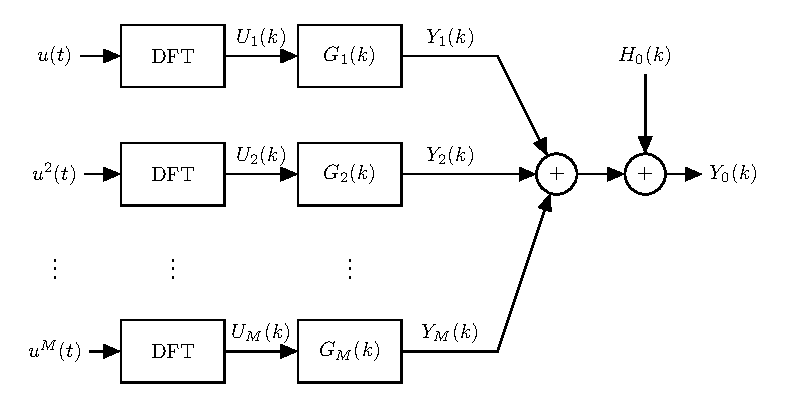
\includegraphics[width=0.9\textwidth]{Chapter3_VolterraSeries/NOFRF_blockstructure.pdf}
\caption{Equivalent block structure of the NOFRF model}
\label{fig:NOFRF_ModelStructure}
\end{figure}

As can be seen in (\ref{eq:GFRF2NOFRF}), the NOFRF series is an input dependent model unlike its GFRF counterpart. The dependence arises because the NOFRFs act on powers of the input rather than the input directly, and this property limits their utility in system analysis. Nevertheless, in Chapter \ref{chap:7} we will examine a special case where the NOFRFs are input independent and pseudo-linear.

\section{Properties and assumptions}
\label{sec:VolterraProperties}

Some important properties and assumptions for Volterra series models will be established in this section and considered true in the sequel. The first of these properties concerns causality.
\begin{defn}[Causal Volterra kernel]
A Volterra kernel $h_m(\tau_1, \hdots, \tau_m)$ is said to be causal if it satisfies
\begin{equation}
h_m(\tau_1, \hdots, \tau_m) = 0 \; \; \forall \tau_i < 0, \; \; \; i = 1, \hdots, m.
\end{equation}
\end{defn}
The implication of causality is that the output contribution produced by a causal kernel cannot be influenced by future input samples.

Another issue which requires careful consideration is the uniqueness of Volterra series models.
\begin{property}
In general, a Volterra kernel $h_m(\tau_1, \hdots, \tau_m)$ is non-unique for $m > 1$, i.e. there are other kernels which will produce the same input to output mapping.
\end{property}
While non-uniqueness is certainly undesirable from an identification standpoint, there is a special subset of kernels which are unique within their set. These are the symmetric Volterra kernels.  
\begin{defn}[Symmetry]
A symmetric kernel $h_m(\tau_1, \hdots, \tau_m)$ is one in which the value of the kernel is independent of the ordering of the lag variables, i.e.
\begin{align}
h_m(\tau_1, \tau_2, \hdots, \tau_m) = h_m(\tau_2, \tau_1, \hdots, \tau_m) = \hdots = h_m(\tau_{i_1}, \tau_{i_2}, \hdots, \tau_{i_m}) \\
i_j \neq i_k, \; \; \; i_1, i_2, \hdots, i_m \in (1,2,\hdots,m) \nonumber
\end{align}
\end{defn}
A symmetric kernel is unique in the sense that there exists no other \emph{symmetric} kernel that exhibits the same input to output mapping. For this reason, assuming symmetry has become the common convention when dealing with Volterra series models \cite{Cheng2017}. Even in the case where an asymmetric kernel is provided, a symmetric kernel can be easily generated \cite{Schetzen1980}.
\begin{property}
Any non-unique asymmetric Volterra kernel $h_m^*(\tau_1, \hdots, \tau_m)$ can be used to generate a unique symmetric equivalent kernel, $h_m$, by averaging all kernels obtained from the set, $S_m$, of all possible permutations of $\bm{\tau}=[\tau_1,\hdots,\tau_m]$, i.e.
\begin{equation}
h_m(\tau_1, \hdots, \tau_m) = \frac{1}{m!} \sum_{\bm{\tau} \in S_m} h_m^*(\bm{\tau}).
\end{equation}
\end{property}

Symmetric kernels not only solve the uniqueness issue for Volterra series, they also reduce the number of parameters to be estimated in a given kernel. Since the order of the lags is not important, we need only identify the parameter once for each combination of lag values, instead of each permutation. As a result, the expression for the number of \emph{unique} parameters requiring estimation in an $m$\textsuperscript{th} order symmetric kernel with memory length $n_m$ is given by,
\begin{equation} 
\label{eq:ParametersPerKernel}
d_m = \binom{n_m+m-1}{m} = \frac{\prod_{i=0}^{m-1}(n_m + i)}{m!}.
\end{equation}
While symmetry does provide a reduction in the number of estimated parameters, the series is still plagued by the `curse of dimensionality', a phrase used to describe the rapid increase in parameter space as problems are moved to higher dimensions. Indeed, (\ref{eq:ParametersPerKernel}) shows the number of parameters will increase exponentially with nonlinear order (dimension) $m$, and combinatorially with memory length $n_m$. This parameter growth is visualized in Figure \ref{fig:ParameterGrowthCurse}.

\begin{figure}[h]
\centering
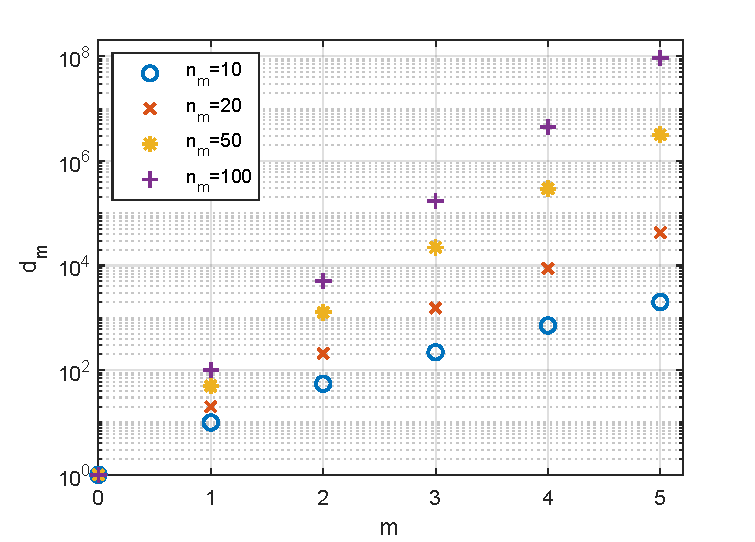
\includegraphics[width=0.65\textwidth]{Chapter3_VolterraSeries/ParameterGrowthB.pdf}
\caption{Number of unique kernel parameters for varying dimension and memory length}
\label{fig:ParameterGrowthCurse}
\end{figure}

The final consideration which must be made is stability. In the case of linear systems, bounded-input bounded-output (BIBO) stability can be defined easily using the impulse response representation. In particular for discrete-time models, a necessary and sufficient condition is that the impulse response be absolutely summable:
\begin{equation}
\sum_{\tau=0}^{\infty} |h(\tau)| < \infty.
\end{equation}
For Volterra series models, the situation is similar but not quite as straightforward. 
\begin{property}
For a causal Volterra kernel $h_m(\tau_1, \hdots, \tau_m)$, the kernel is BIBO stable if
\begin{equation}
\sum_{\tau_1=0}^{\infty} \hdots \sum_{\tau_m=0}^{\infty}|h_m(\tau_1, \hdots, \tau_m)| < \infty.
\end{equation}
\end{property}
The condition that the kernel be absolutely summable is sufficient to give BIBO stability, however it is no longer a necessary condition for $m>1$. Furthermore, a method for constructing stable kernels which violate this condition can be found in \cite{Schetzen1980}. While such special cases exist, in practice one would expect the kernels to decay to zero in all directions of increasing lag, implying that we have absolute summability.

Having established some important properties of the Volterra series and its associated kernels, the following assumption will hold true for the remainder of the thesis.
\begin{assum}
All nonlinear systems considered in this thesis can be represented by Volterra series models which contain causal, symmetric, and absolutely summable kernels.
\end{assum}

\section{Relationship to common block structures}
\label{sec:BlockStructureRelationship}

While block-oriented models are not the focus of this thesis, some of the more common block structures can be related to an equivalent Volterra series representation in an explicit sense. These relationships have been explored in e.g. \cite{Westwick2003} and \cite{Kibangou2010}, and will be used in the sequel to generate simulated Volterra systems with which to test the proposed algorithms. First, some assumptions are placed on the static nonlinear and linear dynamic blocks.

\begin{assum}
\label{assum:polynomialnonlin_Chap3}
In all block structures, the static nonlinear block can be represented by a polynomial nonlinearity\footnote{The polynomial assumption on $F(x(t))$ is not particularly restrictive, since any continuous function can be approximated arbitrarily well (in a least squares sense) over a finite interval by a polynomial of sufficiently high degree \cite{Timan1963}. For discontinuous functions, a similar pointwise convergence can be established as polynomial degree approaches infinity.},
$$F(x(t)) = \beta_0 + \beta_1 [x(t)] + \hdots + \beta_M [x(t)]^M.$$
\end{assum}

\begin{assum}
\label{assum:linearblock_Chap3}
In all block structures, the linear blocks are stable rational filters which can be represented by their corresponding impulse response, $g_i(\tau)$ for some integer subscript $i$.
\end{assum}

With these assumptions in place, three of the most well known block-oriented models are introduced, and their relationship to the Volterra series representation is defined.

\subsection{Wiener model}

The Wiener block structure consists of a single linear filter followed by a static nonlinear block to generate the output. A block diagram is provided in Figure \ref{fig:WienerBS}.

\begin{figure}[!h]
\centering
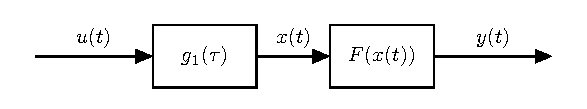
\includegraphics[scale=1]{Chapter3_VolterraSeries/WienerSystem.pdf}
\caption{Block structure for a Wiener model}
\label{fig:WienerBS}
\end{figure}

For the Wiener model, equivalent Volterra kernels are generated as follows,
\begin{align}
h_0 &= \beta_0, \nonumber \\
h_m(\tau_1,\hdots,\tau_m) &= \beta_m \cdot g_1(\tau_1) \cdot \hdots \cdot g_1(\tau_m).
\end{align}

\subsection{Hammerstein model}

The Hammerstein model contains the same two blocks as the Wiener model, but in the opposite order, i.e. a static nonlinear block followed by a linear filter. The structure is represented in Figure \ref{fig:HammersteinBS}.

\begin{figure}[!h]
\centering
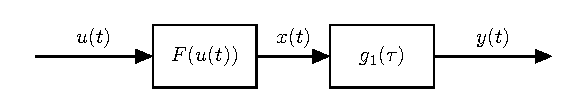
\includegraphics[scale=1]{Chapter3_VolterraSeries/HammersteinSystem.pdf}
\caption{Block structure for a Hammerstein model}
\label{fig:HammersteinBS}
\end{figure}

Hammerstein systems can also be represented using a series of Volterra kernels, i.e.
\begin{align}
h_0 &= \beta_0, \nonumber \\
h_m(\tau_1,\hdots,\tau_m) &= \begin{cases} \beta_m g_1(\tau_1) & \tau_1 = \hdots = \tau_m, \\ 0 & \textrm{otherwise}. \end{cases}
\end{align}
The kernels are seen to be nonzero only on their diagonal elements.

\subsection{Wiener-Hammerstein model}

The Wiener-Hammerstein model has the structure shown in Figure \ref{fig:WienerHammBS}, which is seen to be a combination of the previous two models. In such systems, the static nonlinear block is both preceded and followed by a linear filter. Clearly, Wiener-Hammerstein models are capable of describing a broader range of systems than Wiener and Hammerstein models, since the latter two are just special cases of the former.

\begin{figure}[!h]
\centering
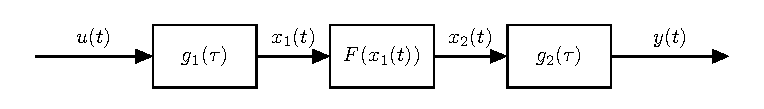
\includegraphics[scale=1]{Chapter3_VolterraSeries/WienerHammSystem.pdf}
\caption{Block structure for a Wiener-Hammerstein model}
\label{fig:WienerHammBS}
\end{figure}

The Volterra kernels corresponding to the Wiener-Hammerstein model are found via
\begin{align}
h_0 &= \beta_0, \nonumber \\
h_m(\tau_1,\hdots,\tau_m) &= \beta_m \sum\limits_{\tau=-\infty}^{\infty} g_2(\tau) \cdot g_1(\tau_1 - \tau) \cdot \hdots \cdot g_1(\tau_m - \tau).
\end{align}

\section{History of Volterra series identification}
\label{sec:VolterraID_History}

Despite the curse of dimensionality, the earliest results on Volterra series identification attempted to use classical methods from statistics involving input-output cross-correlations. Such methods were made more feasible by the development of the Wiener series \cite{Schetzen1974}, which is a variation of the Volterra series that is orthogonal (in discrete-time) for Gaussian white noise input. Estimation of the Wiener series could then be performed individually for each Wiener kernel by computing cross-correlations from experimental data \cite{Lee1965}.

Of course, the assumption of a Gaussian white noise input is too strict to be useful in many practical settings, and significant effort was put towards broadening the applicability of the cross-correlation approach. An extension for coloured (correlated) Gaussian inputs was proposed in \cite{Korenberg1990}, and extensions to other input distributions can be found in \cite{Ogura1972} and \cite{Segall1976}. Despite these efforts, estimation using cross-correlations was not a very efficient tool, requiring very large sample sizes for proper convergence, even in small, low-order problems \cite{Franz2006}.

Apart from using inputs with a known distribution, researchers specifically designed the identification input to maximize the accuracy of their chosen estimator. Some examples of these inputs include pseudorandom binary sequences (PRBS) in \cite{Sutter1987} and \cite{Reed1996}, and pseudorandom multilevel sequences (PRMLS) in \cite{Nowak1994}. These techniques are only applicable if the input used for identification can be precisely controlled, which is not always a realistic assumption.

More recently, the strategy of expanding Volterra series models in terms of a finite set of basis functions has come to the forefront. Such methods can provide a dramatic reduction in the number of parameters requiring estimation, providing the basis functions are chosen appropriately. The earliest examples of this approach appeared in \cite{Amorocho1971} for a hydrologic system, and \cite{Watanabe1975} for a physiological system, which then inspired further results in \cite{Ogura1985} and \cite{Marmarelis1993}. The popularity of the approach gained momentum following papers on the optimal Laguerre \cite{Campello2004} and Kautz \cite{Rosa2007} basis function expansions for Volterra models. As well as the classical sets of orthonormal functions, wavelets have also been explored as a basis due to their desirable properties of orthogonality and compact support \cite{Cheng2017}. Some notable examples can be found in \cite{Nikolaou2000}, \cite{Prazenica2004} and \cite{Prazenica2006}, however these methods are limited to kernels of order three and lower. 

The rapid increase of available computing power in recent decades has allowed more computationally intensive methods to enter the field of Volterra series estimation. A method based on particle swarm optimization was proposed in \cite{Chang2012}, while a relationship between the series and neural networks was discussed in \cite{Wray1994} and used to propose an identification scheme. Regularized linear regression was explored in \cite{Franz2006} using ridge regression. Finally, the Bayesian regularization approach \cite{Birpoutsoukis2017} of interest in this thesis is made possible via intensive global optimization techniques.

The discussion so far has only focussed on time domain estimation, since frequency domain kernels can be obtained indirectly from transformation of the time domain terms. Direct frequency domain estimation has its own history, however, which runs in parallel and follows the same trends as the time domain. Estimation of a system's GFRFs was originally considered for specific and strict experimental conditions. Methods in \cite{Bedrosian1971} required harmonic or Gaussian noise inputs, while \cite{Jones1989} required special harmonic inputs as well as readily available difference equations for the system. Many results employed specially designed periodic multisine inputs, such as \cite{Victor1980}, \cite{Boyd1983}, \cite{Chua1989} and \cite{Evans1996}. More recently, an interpolation method was provided in \cite{Nemeth2002} which exploits the (assumed) local smoothness of GFRFs, and another method has been proposed in \cite{Li2011} which directly uses harmonic time domain data for estimation.       

\section{Regularized Volterra series estimation}
\label{sec:RegVolterraTD}

Inspired by the success of Bayesian regularization techniques in linear impulse response identification \cite{Pillonetto2010}, an extension of the method to the Volterra series was first proposed in \cite{Birpoutsoukis2015}, and further improved in \cite{Birpoutsoukis2017} and \cite{Birpoutsoukis2017c}. The approach is conceptually similar, since each Volterra kernel is a multidimensional impulse response, however the extra dimensions add complexity when designing prior covariances for the kernels. While the properties of smoothness and decay are still integral to the process, they must now be imposed across the entire (hyper)surface of each kernel.

First, assumptions must be placed on the model structure for the system.
\begin{assum}
\label{ass:ReLSmodelstructure}
The system can be represented by a Volterra series model with known deterministic input and white Gaussian measurement noise, $e(t) \sim \mathcal{N}(0,\sigma^2)$, added directly at the output. The measured output, $y$, is then given by 
\begin{equation}
\label{eq:ReLS_VolterraModelStructure}
y(t) = y^0(t) + e(t),
\end{equation} 
where $y^0(t)$ is the noise-free Volterra series output from (\ref{eq:VolterraTimeDomainOutput}). 
\end{assum}

From the assumed model structure, a linear regression formulation of the problem can now be considered, i.e.
\begin{equation}
\label{eq:VolterraRegressionForm}
Y = \Phi^T \theta + E,
\end{equation}
where $Y, E \in \mathbb{R}^{N-n+1}$ are the vectors of output measurements and measurement noise respectively, and $\theta = [h_0, {h_1^\mathcal{V}}^T, {h_2^\mathcal{V}}^T, \hdots, {h_M^\mathcal{V}}^T]^T \in \mathbb{R}^D$ is the parameter vector containing all unique coefficients for each Volterra kernel. For the multi-dimensional kernels, $h_m^\mathcal{V} \in \mathbb{R}^{d_m}$ refers to a vector containing the unique kernel coefficients in $h_m(\tau_1,\hdots, \tau_m)$. The regressor matrix, $\Phi \in \mathbb{R}^{D \times (N-n+1)}$, should be constructed based on the vectorization scheme used in $\theta$, and must take into account the assumed symmetry of kernels in the series. While each kernel's coefficients are free to be ordered in an arbitrary fashion, a structured approach to vectorization is detailed in \cite{Birpoutsoukis2017} for the second order case. A small illustrative example will be given here.   

Consider a 2\textsuperscript{nd} order Volterra series model, with memory lengths ${n_1=n_2=n=3}$ for the kernels. The parameters requiring estimation in this model are depicted in Figure \ref{fig:VolterraRegressionExample}, where black circles indicate unique coefficients to be estimated, and red circles indicate non-unique coefficients which will be estimated. The gray dashed circles give the non-unique coefficients which will not be estimated, but rather inferred using their symmetrical red counterparts. The resulting regression structure is then given by,
\begin{figure}[t]
\centering
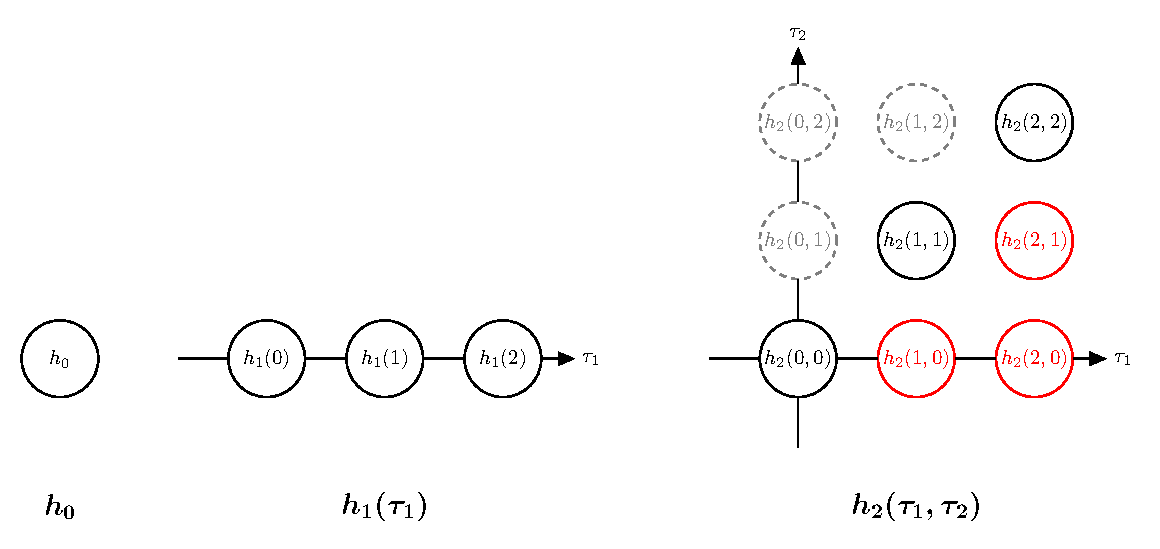
\includegraphics[width = 0.95\textwidth]{Chapter3_VolterraSeries/VolterraSeriesRegressionExample.pdf}
\caption{Estimation parameters in a 2\textsuperscript{nd} order Volterra series with memory length 3}
\label{fig:VolterraRegressionExample}
\end{figure}
\begin{equation*}
\begin{bmatrix} y(2) \\ y(3) \\ \vdots \\ y(N-1) \end{bmatrix} = 
\begin{bmatrix} 1 & 1 & \hdots & 1 \\ u(2) & u(3) & \hdots & u(N-1) \\ u(1) & u(2) & \hdots & u(N-2) \\ u(0) & u(1) & \hdots & u(N-3) \\
u(2) \cdot u(2) & u(3) \cdot u(3) & \hdots & u(N-1) \cdot u(N-1) \\ \textcolor{red}{2} u(1) \cdot u(2) & \textcolor{red}{2} u(2) \cdot u(3) & \hdots & \textcolor{red}{2} u(N-2) \cdot u(N-1) \\
\textcolor{red}{2} u(0) \cdot u(2) & \textcolor{red}{2} u(1) \cdot u(3) & \hdots & \textcolor{red}{2} u(N-3) \cdot u(N-1) \\ u(1) \cdot u(1) & u(2) \cdot u(2) & \hdots & u(N-2) \cdot u(N-2) \\
\textcolor{red}{2} u(0) \cdot u(1) & \textcolor{red}{2} u(1) \cdot u(2) & \hdots & \textcolor{red}{2} u(N-3) \cdot u(N-2) \\ u(0) \cdot u(0) & u(1) \cdot u(1) & \hdots & u(N-3) \cdot u(N-3) \end{bmatrix}^T  
\begin{bmatrix} h_0 \\ h_1(0) \\ h_1(1) \\ h_1(2) \\ h_2(0,0) \\ \textcolor{red}{h_2(1,0)} \\ \textcolor{red}{h_2(2,0)} \\ h_2(1,1) \\ \textcolor{red}{h_2(2,1)} \\ h_2(2,2) \end{bmatrix} + E.
\end{equation*}
Note the non-unique coefficients (highlighted in red) in the parameter vector, which have their regressor entries multiplied by 2 since they represent the contribution of 2 symmetric coefficients in the second order kernel.

Given the model structure assumption in (\ref{eq:ReLS_VolterraModelStructure}), it was shown in Chapter \ref{chap:2} that both the least squares and maximum likelihood estimate of $\theta$ will be given by the analytic solution,
\begin{equation}
\label{eq:LSestimator_VolterraSeries}
\hat{\theta}_{LS} = (\Phi \Phi^T)^{-1} \Phi Y.
\end{equation}

Since the least squares estimation problem is likely to be ill-conditioned or even underdetermined for a Volterra model with large numbers of parameters, we regularize the estimate with a Bayesian-tuned quadratic penalty. The Bayesian method proposed in \cite{Birpoutsoukis2017} treats each Volterra kernel in the model as an independent Gaussian process with a separate prior covariance, outlined in the following assumption.
\begin{assum}[Gaussian priors]
Every vector of kernel coefficients, $h_m^\mathcal{V}$, is a zero mean Gaussian process: 
\begin{equation}
h_m^\mathcal{V} \sim \mathcal{N}(0,P_m) \; \; \; m = 1, \hdots, M.
\end{equation}
Furthermore, all pairs of coefficient vectors, $h_i^\mathcal{V}$ and $h_j^\mathcal{V}$, are independent for $i \neq j$.

The constant offset is also Gaussian, i.e. $h_0 \sim \mathcal{N}(0,P_0)$, and is independent of all other kernels.
\end{assum}

This Bayesian assumption frames the total parameter vector as a Gaussian process, i.e. $\theta \sim \mathcal{N}(0,P)$, where $P$ is the total prior covariance constructed as a block diagonal matrix,
\begin{equation}
\label{KernelPenalty}
P = \begin{bmatrix}
       P_0 & & &  \multirow{2}{*}{\huge 0} \\
       & P_1 & & \\
      \multirow{2}{*}{\huge 0} & & \ddots & \\
       &  & & P_M
     \end{bmatrix},
\end{equation}
with $P_m \in \mathbb{R}^{d_m \times d_m}$ being the prior covariance for the $m$\textsuperscript{th} Volterra kernel. 

Individually, the prior covariance matrices should be designed to impose smoothness and exponential decay on their multi-dimensional kernels, as in the FIR case. For $P_1$, the TC structure in (\ref{eq:TCstructure}) or DC structure in (\ref{eq:DCstructure}) can be directly applied, since $h_1$ is effectively an impulse response. For kernel dimensions greater than one, the TC or DC structure must be incorporated into a more complex covariance matrix in order to impose smoothness and stability along the entire (hyper)surface. The approach suggested in \cite{Birpoutsoukis2017} is to consider $m$ perpendicular regularizing directions for the kernel $h_m$, where the vector $(1,\hdots,1)$ is always included as one of the directions. As an example, the regularizing directions for a second order kernel are shown in Figure \ref{fig:SecondOrderRegDir}. A rotated coordinate system can be formed from the set of regularizing vectors, which we will denote $(v_m^1, \hdots, v_m^m)$.  

\begin{figure}[h]
\centering
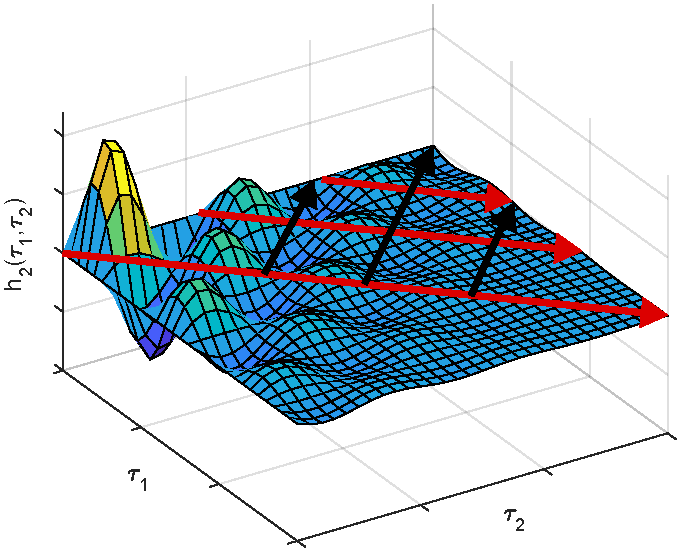
\includegraphics[width = 0.6\textwidth]{Chapter3_VolterraSeries/RegDirections3.pdf}
\caption{The two perpendicular regularizing directions, (1,1) (red) and (-1,1) (black), for a second order Volterra kernel}
\label{fig:SecondOrderRegDir}
\end{figure}

\begin{rem}
A suitable set of orthogonal regularizing directions for the $m$\textsuperscript{th} nonlinear order can be obtained via the following standard form (for $m \geq 3$):
\begin{equation}
\begin{split}
v_m^1 &= (1,1,\hdots,1), \\
v_m^2 &= (-1,\hdots,-1,m-1) \\
v_m^3 &= (-1,\hdots,-1,m-2,0) \\
&\hdots \\
v_m^m &= (-1,1,0,\hdots,0)
\end{split}
\end{equation}
\end{rem}

The rotated coordinate system is used to apply the chosen covariance structure along each regularizing direction, forming a set of $m$ partial covariance matrices. For the regularizing direction $v_m^j$, the corresponding partial covariance matrices for the TC and DC structures are,
\begin{align}
\label{TCext}
&\textbf{TC structure:} \hfill &P_m^j(x,y) = (\lambda_m^j)^{max(x',y')}, \\
&\textbf{DC structure:} \hfill &P_m^j(x,y) = (\lambda_m^j)^{(x' + y')/2} (\rho_m^j)^{|x'-y'|},
\label{DCext}
\end{align}
where $x'$ is the coordinate of $h^{\mathcal{V}}_{m}(x)$ on the $v_m^j$ axis. If $h^{\mathcal{V}}_{m}(x)$ is associated with lag values $\bm{\tau} = (\tau_1, \hdots, \tau_m)$, then $x' = \langle \bm{\tau} , v_m^j \rangle$. An Hadamard product of the partial covariances is required to produce the total prior covariance for the kernel, i.e.
\begin{equation}
\label{FinalPenalty}
P_m = c_m \cdot P_m^1 \circ \hdots \circ P_m^m, \; \; \; \; m = 1, \hdots, M.
\end{equation}
where $c_m$ is a normalization hyperparameter. The covariance for $h_0$ is simply given by 
\begin{equation}
P_0 = c_0.
\end{equation}

There are clearly a large number of hyperparameters which require empirical tuning to form our regularization penalty, $P$. More specifically, there are $m+1$ hyperparameters per kernel when using a TC structure, which include the normalization constant, $c_m$, and $m$ decay constants, $\lambda_m^j$. Using the DC structure increases this to $2m+1$ hyperparameters per kernel, by including the $\rho_m^j$ set. In either case, the suggested method for hyperparameter tuning in \cite{Birpoutsoukis2017} is to use the standard marginal likelihood maximization of (\ref{eq:MarginalLikelihood_opt}). While the optimization is still applicable in the Volterra series case, the large dimension of the search space and non-convexity of the problem can yield prohibitively long computation times, with a high risk of settling in sub-optimal local minima. These complications motivate the research in Chapter \ref{chap:4} of this thesis.

Following the hyperparameter tuning (which may also include noise variance $\sigma^2$), $P$ can be constructed, and the regularized estimate of $\theta$ may be obtained analytically from (\ref{eq:MLE_BayesianRegularization}).

As an illustration of the profound benefit of Bayesian regularization in Volterra series estimation, parameter estimates have been obtained for a simple 2\textsuperscript{nd} order example system, whose true kernels are shown in Figure \ref{fig:ExampleLSvsReLS_TrueKernels}. Estimates of these kernels were obtained using 
\begin{enumerate}
\item A simple least squares estimator (\ref{eq:LSestimator_VolterraSeries})
\item A regularized estimate (\ref{eq:MLE_BayesianRegularization}) with empirically tuned TC structure for $P$ via (\ref{KernelPenalty}), (\ref{TCext}) and (\ref{eq:MarginalLikelihood_opt})
\end{enumerate}

\begin{figure}[h]
\centering
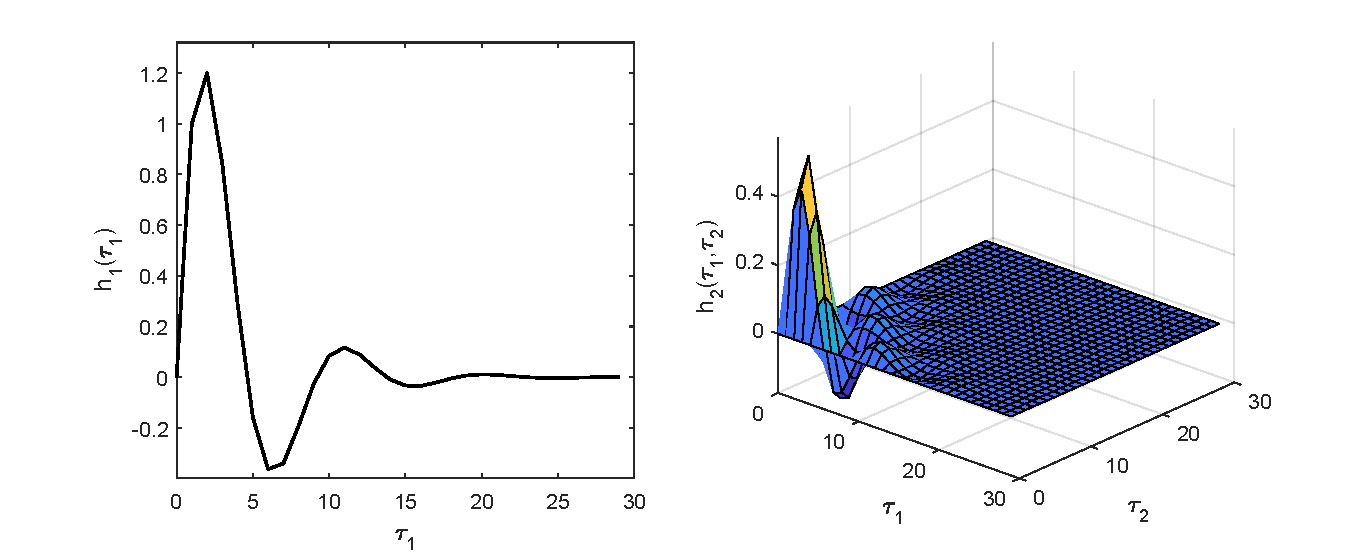
\includegraphics[width = 1\textwidth]{Chapter3_VolterraSeries/LSvsReLS_truekernels.pdf}
\caption{True Volterra kernels for the comparative simulation example}
\label{fig:ExampleLSvsReLS_TrueKernels}
\end{figure}

The first set of estimates, shown in Figure \ref{fig:ExampleLSvsReLS_VolterraSeries2_whitenoise}, were obtained from a simulation of the system in Figure \ref{fig:ExampleLSvsReLS_TrueKernels} for a dataset with length $N=1000$, noise variance $\sigma^2 = 1$, and a white Gaussian noise input. In this case, the input signal is sufficiently exciting, however the least squares estimate still suffers from high covariance due to the large number of parameters being estimated. The regularized estimator, however, produces smooth, accurate estimates of the Volterra kernels due to the construction of prior covariances which impose the desired behaviour. 

The second set of estimates, shown in Figure \ref{fig:ExampleLSvsReLS_VolterraSeries2_filterednoise}, were obtained using the same specifications, except that the input is now \emph{filtered} Gaussian noise. In this case the input does not have energy in the full frequency band (i.e. it is not sufficiently exciting), hence the least squares estimator is ill-conditioned and the resulting estimate is unusable. The regularized estimate, on the other hand, is relatively unaffected by the change. 

\vspace{10mm}

\begin{figure}[!hp]
\centering
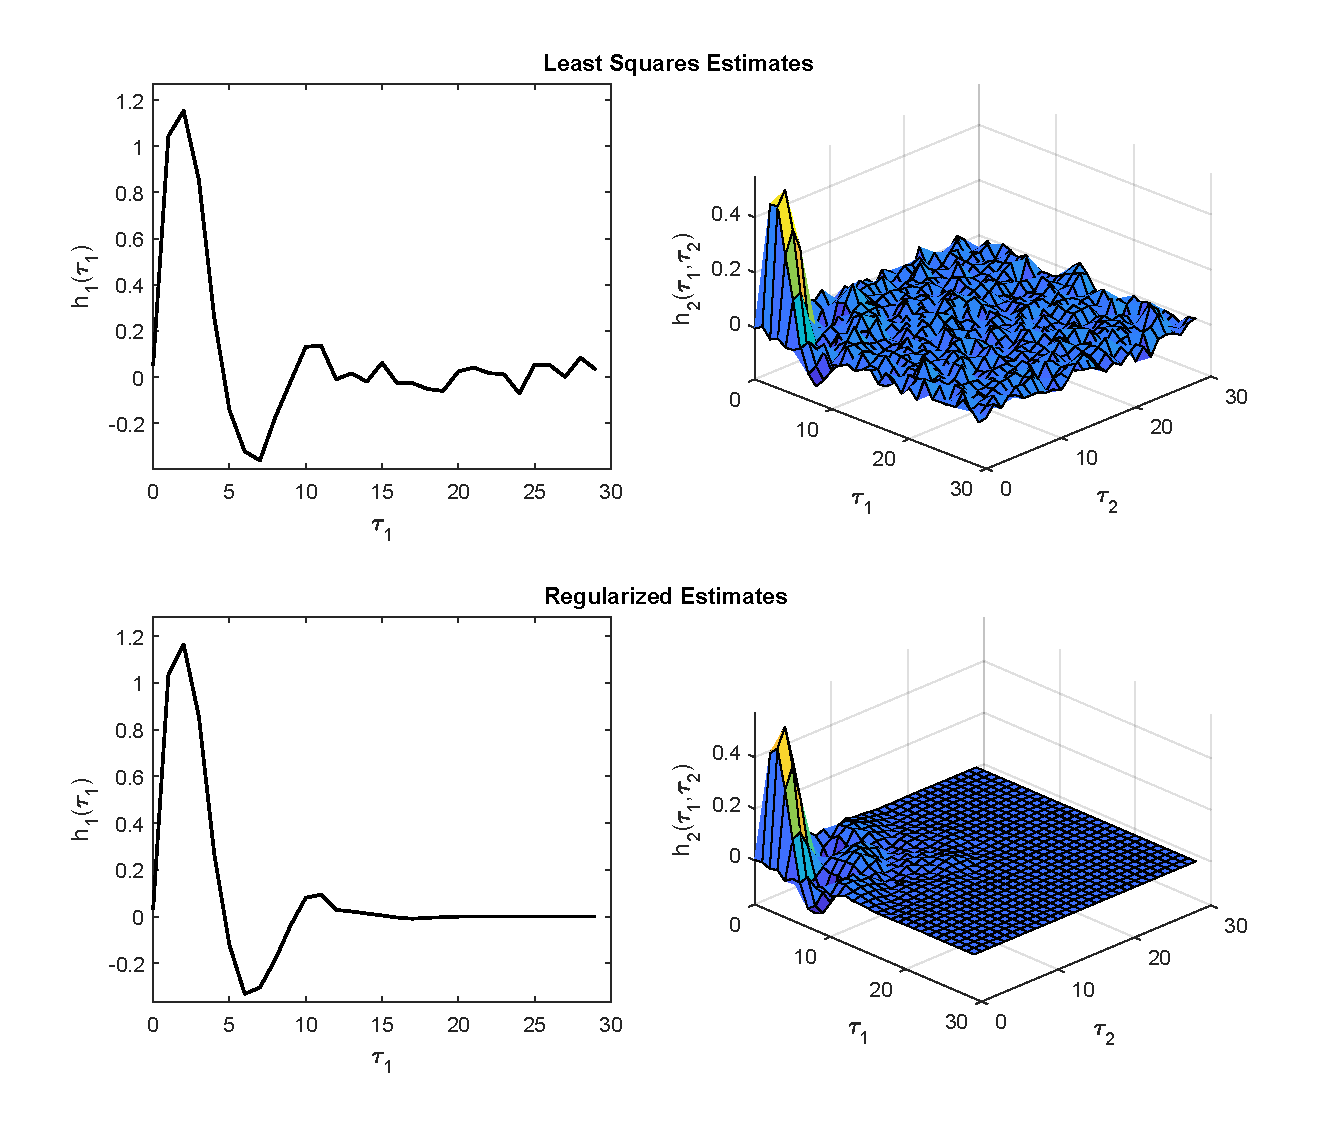
\includegraphics[width = 1.1\textwidth]{Chapter3_VolterraSeries/LSvsReLS_whiteinput.pdf}
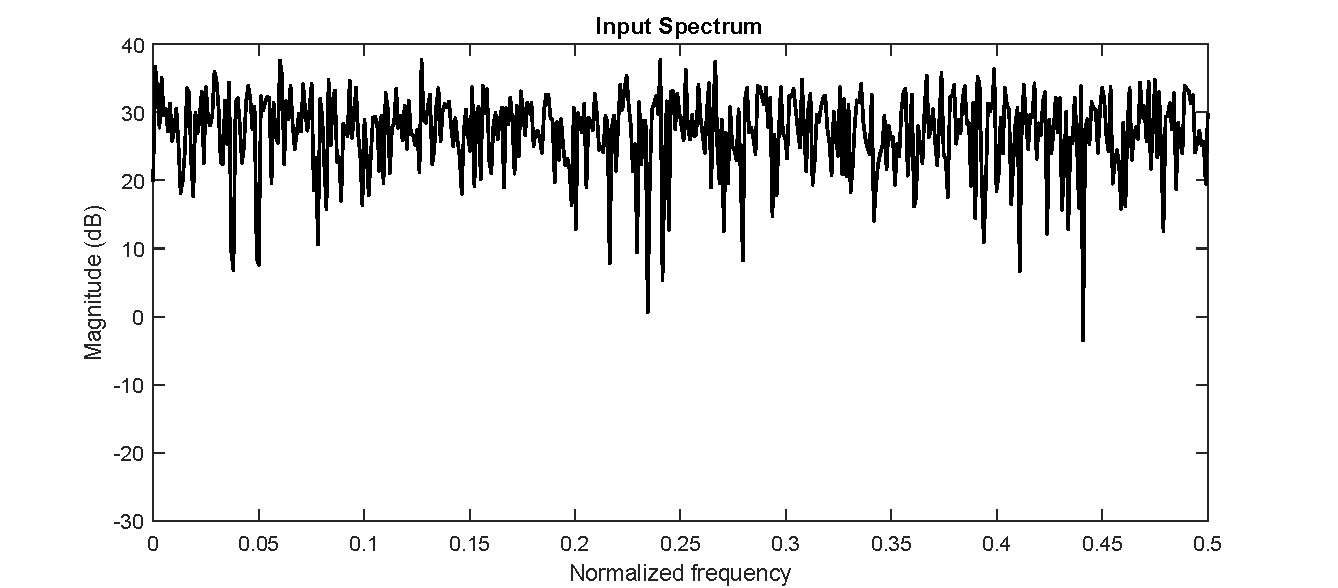
\includegraphics[width = 1.1\textwidth]{Chapter3_VolterraSeries/white_spectrum.pdf}
\caption{Least squares (top) and regularized (middle) kernel estimates for a white Gaussian input (bottom)}
\label{fig:ExampleLSvsReLS_VolterraSeries2_whitenoise}
\end{figure}

\begin{figure}[!hp]
\centering
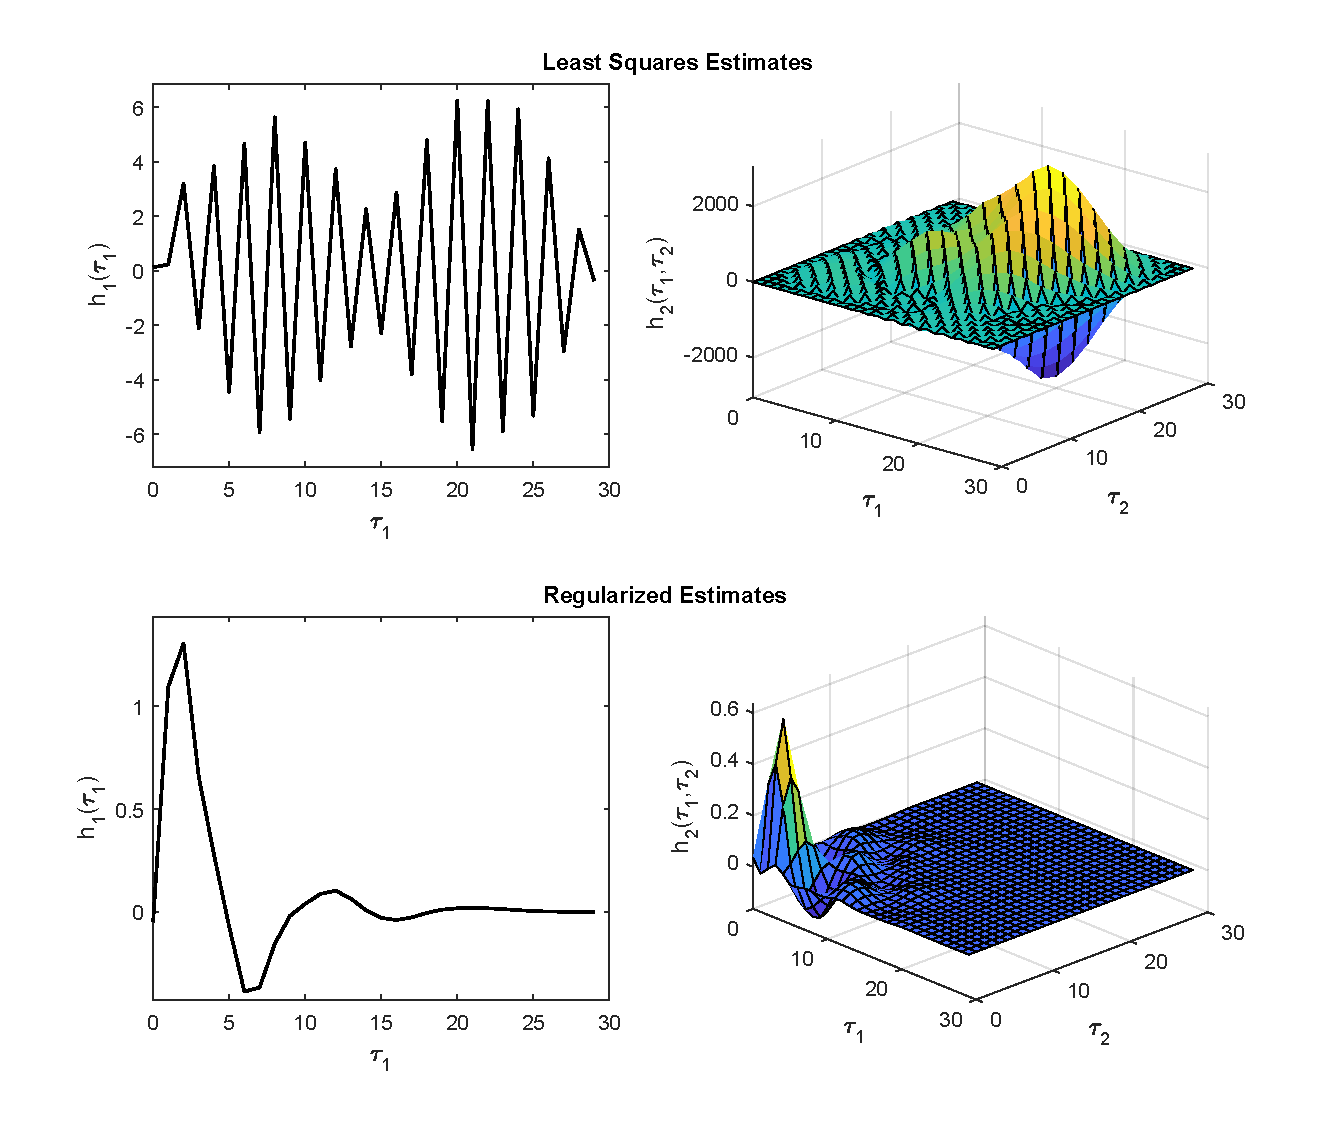
\includegraphics[width = 1.1\textwidth]{Chapter3_VolterraSeries/LSvsReLS_butterworthinput.pdf}
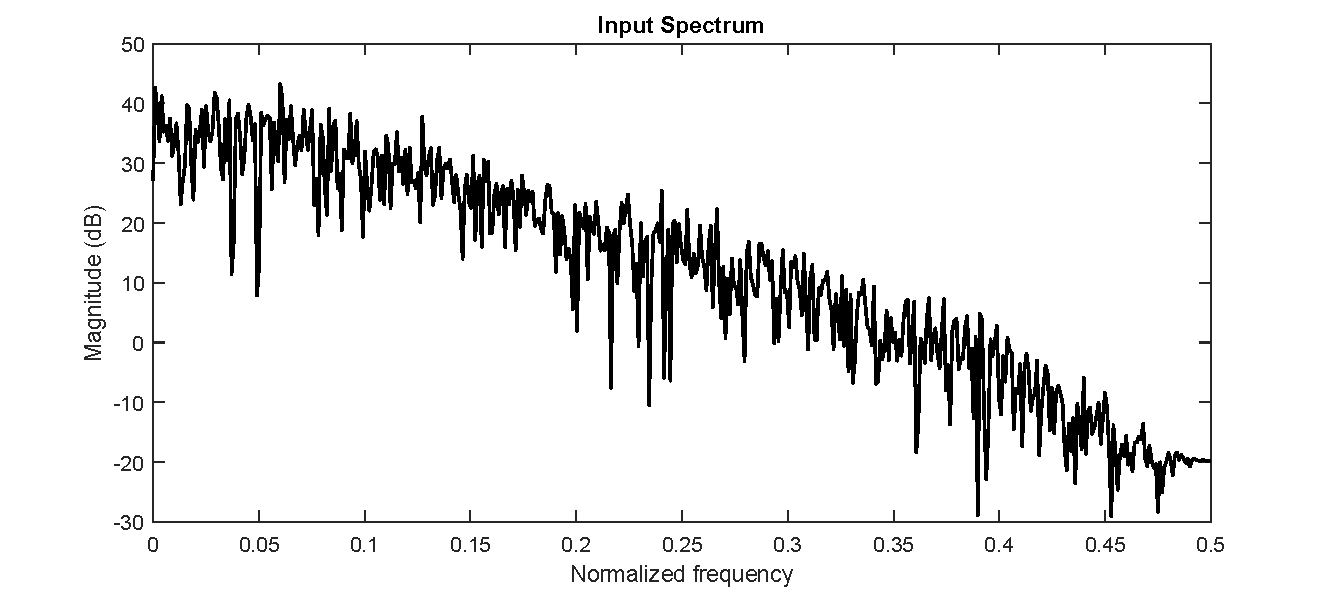
\includegraphics[width = 1.1\textwidth]{Chapter3_VolterraSeries/butterworth_spectrum.pdf}
\caption{Least squares (top) and regularized (middle) kernel estimates for a filtered Gaussian input (bottom)}
\label{fig:ExampleLSvsReLS_VolterraSeries2_filterednoise}
\end{figure}
 
\section{Summary}
 
The Volterra series model for nonlinear dynamical systems was introduced in this chapter, with discrete-time representations defined in both the time and frequency domain. Assumptions of causality, stability and symmetry were established for each Volterra kernel in the series, and the parameter growth issue (i.e. the curse of dimensionality) was discussed. Previous results on the identification of Volterra series models were summarized, and particular attention was paid to the Bayesian regularization method proposed recently in the literature. The regularized approach was developed for time domain identification, and will serve as a foundation for the extensions proposed in Part \ref{part:TD} of this thesis, as well as inspiration for many of the frequency domain contributions in Part \ref{part:FD}.